% Preamble
\documentclass[10pt,twoside,b5paper]{book}

% Packages
\usepackage{lipsum}
\usepackage{graphicx}
\usepackage{xcolor}
\usepackage{datetime}
\usepackage[scaled]{helvet}
%\newdateformat{specialdate}{\twodigit{\THEDAY} \ \monthname[\THEMONTH] \THEYEAR}
\newdateformat{specialdate}{\THEDAY \ \monthname[\THEMONTH] \THEYEAR}
%\usepackage[showframe=true,top=1cm,bottom=1cm,left=1cm,right=1cm]{geometry}
\usepackage[top=3cm,bottom=2cm,left=2cm,right=2cm]{geometry}

\usepackage{tikz}
\usetikzlibrary{automata, positioning}

\usepackage[pdfusetitle]{hyperref}

\usepackage[T1]{fontenc}
\renewcommand\familydefault{\sfdefault}

\author{Joshua David Springer}
\title{Autonomous Precision Drone Landing on Marked Landing Pads and Solidified Lava Flows}
\date{\specialdate\today}

\begin{document}

	\frontmatter
	\noindent 
\thispagestyle{empty}
\begin{center}
\begin{minipage}{0.80\linewidth}
	\centering
	% University logo
	
\includegraphics[width=0.35\linewidth]{./images/ru_logo_transparent}
	\par
	% Title
	\maketitle
    \vskip\baselineskip
    {\author}
% Degree
Dissertation submitted to the School of Computer Science \\ 
at Reykjavík University in partial fulfillment \\
of the requirements for the degree of \\
\textbf{Doctor of Philosophy}\par

\end{minipage}
\end{center}

\vspace{1cm}
\noindent
\begin{center}
\begin{minipage}{0.80\linewidth}
\begin{tabular}{lll}
\textbf{Supervisor:} & Marcel Kyas & Reykjavík University, Iceland\\
	\textbf{Internal Examiner:} & Joseph Timothy Foley & Reykjavík University, Iceland\\
\textbf{Internal Examiner:} & Gylfi Þór Gúðmundsson & Reykjavík University, Iceland\\
\textbf{External Examiner:} & Sebastian Scherer & Carnegie Mellon University\\ 
\end{tabular}
\end{minipage}
\end{center}

\clearpage

	\noindent This manuscript has been read and accepted for the Graduate Faculty in
Computer Science in satisfaction of the dissertation requirements for the
degree of Doctor of Philosophy.

\bigskip

\hfill {Date of Signature}

\vspace{1.5\baselineskip}

\noindent\rule{3.5in}{0.7pt} \hfill \rule{1in}{0.7pt}

\noindent Marcel Kyas\\
Assistant Professor, Department of Computer Science\\ Reykjavik, Iceland
\vspace{1.5\baselineskip}

\noindent\rule{3.5in}{0.7pt} \hfill \rule{1in}{0.7pt}

\noindent Joseph Timothy Foley\\
Assistant Professor, Department of Engineering\\ Reykjavik, Iceland
\vspace{1.5\baselineskip}

\noindent\rule{3.5in}{0.7pt} \hfill \rule{1in}{0.7pt}

\noindent Gylfi Þor Guðmundsson\\
Adjunt Professor, Department of Computer Science\\Reykjavik, Iceland \par
\vspace{1.5\baselineskip}
\noindent\rule{3.5in}{0.7pt} \hfill \rule{1in}{0.7pt}

\noindent Sebastian Scherer,\\
Carnegie Mellon University\\Pittsburgh, Pennsylvania \\ 
\vspace{1\baselineskip}

\clearpage


	\tableofcontents
	\newpage
	

	\mainmatter
	\chapter{Introduction}
		This is a \LaTeX template document.\cite{small}

\begin{figure}
    \centering
    \includegraphics[width=0.5\textwidth]{example-image-a}
\end{figure}

		\newpage

		\section{Acknowledgements}
		\lipsum[5-6]

		\newpage

		\section{Abstract}
		\maketitle
\lipsum[0-1]

		\newpage

		\section{Abstrakt á Íslensku}
		\maketitle
\lipsum[5-6]

		\newpage

		\section{Overview}
		This section outlines the overall story of the PhD,
which originates with the author's master project.
We discuss the motivations for each step of the research,
and the conditions for transitioning between each.

\begin{center}
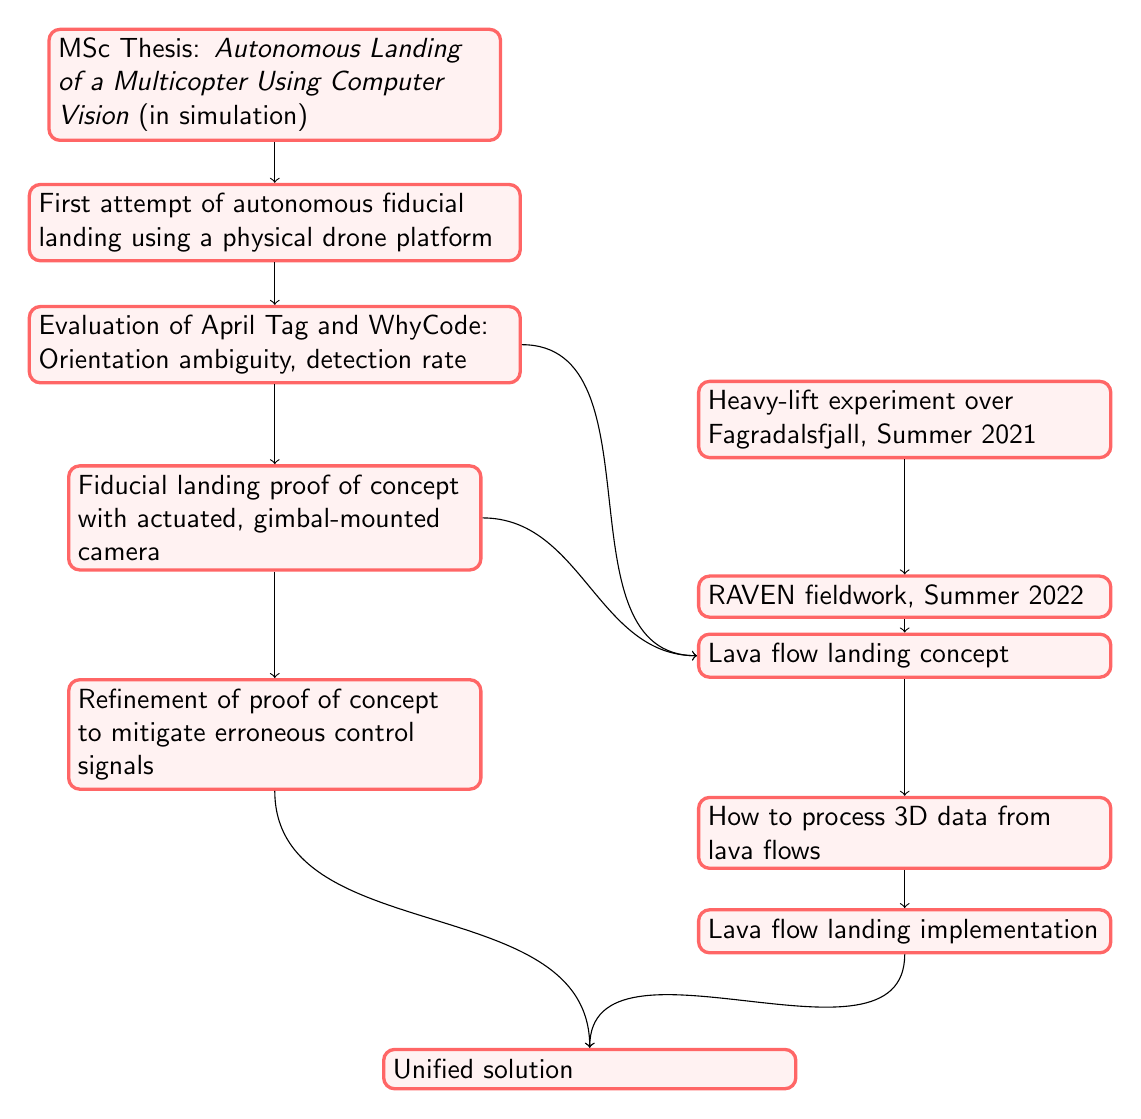
\begin{tikzpicture}[
roundnode/.style={circle, draw=green!60, fill=green!5, very thick, minimum size=7mm},
squarednode/.style={rounded corners, draw=red!60, fill=red!5, very thick, minimum size=5mm},
]
%Nodes
\node[squarednode, text width=5.5cm] (msc) at (0,0) { MSc Thesis: \emph{Autonomous Landing of a Multicopter Using Computer Vision} (in simulation) };
\node[squarednode, text width=6cm] (first_attempt) at (0,-1.75) { First attempt of autonomous fiducial landing using a physical drone platform };
\node[squarednode, text width=5cm] (raven_fagradalsfjall) 	at (8,-4.25) 	{ Heavy-lift experiment over Fagradalsfjall, Summer 2021 };
\node[squarednode, text width=6cm] (evaluation) 		at (0,-3.3) 	{ Evaluation of April Tag and WhyCode: Orientation ambiguity, detection rate};
\node[squarednode, text width=5cm] (poc) 			at (0,-5.5) 	{ Fiducial landing proof of concept with actuated, gimbal-mounted camera };
\node[squarednode, text width=5cm] (raven_fieldwork_2022)	at (8,-6.5)	{ RAVEN fieldwork, Summer 2022 };
\node[squarednode, text width=5cm] (lava_landing_concept)	at (8, -7.25)	{ Lava flow landing concept };
\node[squarednode, text width=5cm] (refinement)			at (0,-8.25)	{ Refinement of proof of concept to mitigate erroneous control\\signals };
\node[squarednode, text width=5cm] (lava_processing)		at (8,-9.5)	{ How to process 3D data from lava flows };
\node[squarednode, text width=5cm] (lava_landing_implementation)		at (8,-10.75)	{ Lava flow landing implementation };
\node[squarednode, text width=5cm] (unified)		at (4,-12.5) 	{ Unified solution };

%Lines
\draw[->] (msc.south) -- (first_attempt.north);
\draw[->] (first_attempt.south) -- (evaluation.north);
\draw[->] (raven_fagradalsfjall.south) -- (raven_fieldwork_2022.north);
\draw[->] (evaluation.south) -- (poc.north);
\draw[->] (poc.south) -- (refinement.north);
\draw[->] (refinement.south) to [out=270,in=90] (unified.north);
\draw[->] (raven_fieldwork_2022.south) -- (lava_landing_concept.north);
\draw[->] (lava_landing_concept.south) -- (lava_processing.north);
\draw[->] (lava_processing.south) -- (lava_landing_implementation.north);
\draw[->] (lava_landing_implementation.south) to [out=270,in=90] (unified.north);
\draw[->] (evaluation) to [out=0,in=180] (lava_landing_concept);
\draw[->] (poc) to [out=0,in=180] (lava_landing_concept);


\end{tikzpicture}
\end{center}

		\newpage

	\chapter{Structured Landing Sites with Fiducial Markers}
		\section{Overview}
		\section{Fiducial System Tests and Modifications}
		\section{First Autonomous Landing Setup}
		\section{Improved Autonomous Landing Setup}

	\chapter{Viable Landing Sites in Solidified Lava Flows}
		\section{Overview}
		\section{RAVEN Fieldwork, Summer 2022}
		\section{Bolluhraun Fieldwork}
		\section{Viable Landing Site Detection}

	\bibliography{references}
	\bibliographystyle{plain}

\end{document}
